Before performing physics measurements, a detailed characterization of both scintillators and electronics modules is necessary, in order to identify possible systematic uncertainty sources then employ reasonable corrections to measures afterward. Moreover, further reasons to fully benefit from this investigation are certainly given by the need to choose an optimized setup of the instrumentation and by the importance of comprehending instruments responses.

\section{Electronics modules characterization}
\subsection{Discriminator} \label{discriminator}
The first module (not incorporated in the detector structure) involved in pulse processing is the discriminator whose input is a linear pulse, while its output is a logic pulse. Among several kinds of triggering, a \emph{leading edge} one has been used, so that the logic pulse is provided when the input exceeds a fixed discrimination level.\\

In particular a \textbf{CAEN N.147 8-Channel Low-Threshold Discriminator} (see Appendix \ref{app:discriminator}) has been employed: 7 of 8 channels have been studied (as the last channel was damaged) by means of a square-pulses generator, in order to determine possible shifts between threshold values measured with a tester and the actual ones, inferred by sending to the channel-input a series of different amplitude pulses. The procedure provides for a gradual increase of the input amplitude up to the first value that corresponds to a non-flat output: that value is the experimental threshold voltage. This process has been repeated for several thresholds\footnote{The trigger level is adjustable by turning a screw.}: no relevant differences between tester values and experimental threshold levels have been observed (up to electronics noise fluctuations).\\

The discriminator gives also the possibility to vary the output duration (by turning a specific screw) and this feature turns out to be fundamental in avoiding a not-negligible source of systematic errors (see Subsection \ref{sub:detection_eff}).
\begin{figure}[!htp]
	\centering
	\begin{subfigure}{.3\linewidth}
		\centering
		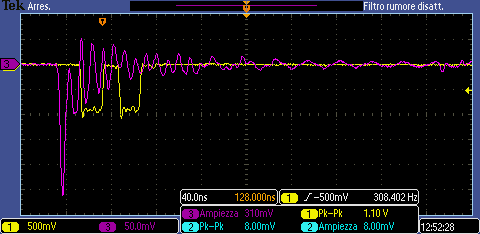
\includegraphics[width=\linewidth]{characterization/double}
		\caption{Wrong double output generation.}
		\label{subfig:double}
	\end{subfigure}\hfill
	\begin{subfigure}{.3\linewidth}
		\centering
		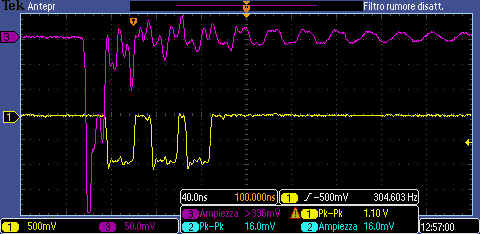
\includegraphics[width=\linewidth]{characterization/triple}
		\caption{Wrong triple output generation.}
		\label{subfig:triple}
	\end{subfigure}\hfill
	\begin{subfigure}{.3\linewidth}
		\centering
		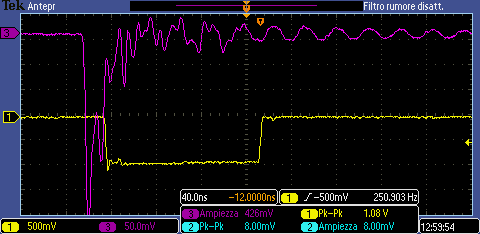
\includegraphics[width=\linewidth]{characterization/single}
		\caption{Correct single output generation.}
		\label{subfig:single}
	\end{subfigure}
	\caption{Oscilloscope visualization. The purple lines represents \emph{Cerbero} anodic outputs, while the yellow ones are the logic pulses provided by the discriminator.}
	\label{fig:window}
\end{figure}
Problems arise when a quite low trigger voltage is combined with an input pulse affected by an important noise level: one is able to note by observing Figures \ref{subfig:double} and \ref{subfig:triple} how this situation could lead to the generation of more than one output pulses per single input, due to a too small time-window. This behavior certainly represents a problem when counting experiments are carried out. Since the discriminator is not able to provide a new pulse when the previous one is still ongoing, the problem is satisfactorily solved by widening the time-window up to the typical duration of the input signal (Figure \ref{subfig:single}).

This kind of issue has not been observed in the less noisy \emph{Minosse} and \emph{Caronte} detectors, but, as a preventive action, the corresponding discriminator outputs duration is set according to what explained above.

\begin{table}[!htp]
	\centering
	\begin{tabular}{cc}
		\toprule
		Detector	&	Time-window $(\si{\nano\second})$ \\
		\midrule
		\emph{Caronte}	&	$40$ \\
		\emph{Cerbero}	&	$80$ \\
		\emph{Minosse}	&	$40$ \\
		\bottomrule		
	\end{tabular}
	\caption{Discriminator output time-windows.}
	\label{window}
\end{table}

A side effect of a larger time-window is the growth of the measure dead-time, but this does not create a problem in muons lifetime measurements. As a matter of fact the expected cosmic muons rate at the ground\footnote{According to \eqref{mu-rate} the expected muon rate per surface unit at the ground is equal to $\approx 1\,\si{cm^{-2}} \,\si{min^{-1}}$ (for a thin horizontal detector), which provides a rate of about $\SI{40}{\hertz}$ relative to the involved detectors.} is $\approx \SI{40}{\hertz}$: this means that two consecutive muons are averagely time-separated by
\begin{displaymath}
\langle t \rangle  = \frac{1}{\langle \Gamma \rangle} \approx \frac{1}{\SI{40}{\hertz}}=2.5\cdot 10^7\,\si{\nano\second}\gg \SI{80}{\nano\second}.
\end{displaymath}

\subsection{Delay unit}
When configuring the electronic chain setup, the delays between different signals have to be kept under control, for the purpose of a correct pulse processing: this goal is achieved by employing LEMO cables of suitable lengths and/or using a delay unit. The latter is a passive module as it do not need a power supply, therefore the delay is realized in a very simple way, by letting the signal pass through internal cables from input to output.\\

The matter is to verify to what extent the nominal delay matches the experimental one.  
\begin{figure}[!h]
	\centering
	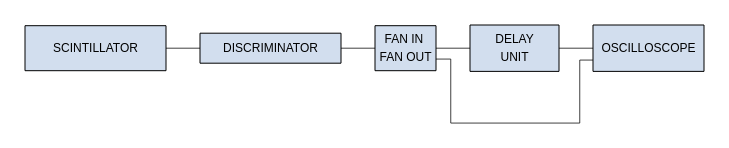
\includegraphics[width=.8\linewidth]{characterization/delay}
	\caption{Configuration employed during delay unit characterization.}
	\label{fig:delay}
\end{figure}
The setup in Figure \ref{fig:delay} shows how the delay can be directly observed measured. Although one could measure by means of oscilloscope's cursors the input/output phase shift induced by \textbf{CAEN N. 108 Dual Delay}, a more systematic approach\footnote{The waveforms have not been observed to be static, instead they are subject to small fluctuations, thus several signals have been acquired.} has been preferred. Both input and output waveforms are displayed in an oscilloscope and acquired (15 for each nominal delay) so as to perform offline analyses.
\begin{figure}[!h]
	\centering
	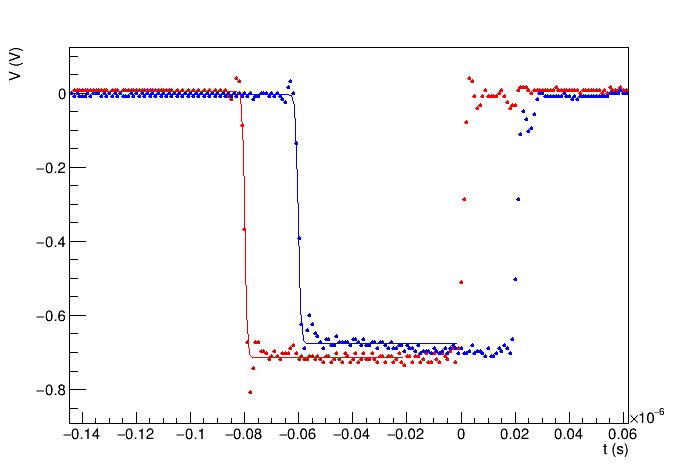
\includegraphics[width=.75\linewidth]{characterization/FD_20ns}
	\caption{Input (red) and output (blue) waveforms corresponding to $\SI{20}{\nano\second}$ nominal delay.}
	\label{fig:wf}
\end{figure}
Most difficulties are given by the limited sampling rate $(\SI{1}{\giga\hertz})$, compared with the rise-time of the square pulses (see Figure \ref{fig:wf} for instance), then, in order to use a reasonable number of points, waveforms are fitted with \emph{Fermi-Dirac}-like functions
\begin{equation} \label{eq:FD}
V(t)=\frac{\alpha}{1+e^{\beta\left(t-\gamma\right)}}+\delta
\end{equation}
where $\alpha,\beta,\gamma,\delta$ are parameters. \eqref{eq:FD} is then inverted
\begin{equation}
t(V) = \frac{1}{\beta}\cdot\ln\left(\displaystyle\frac{\alpha}{V-\delta}-1  \right)+\gamma
\end{equation}
and the experimental delay $\Delta t_{exp}$ is determined as
\begin{equation}
\Delta t_{exp} = t_{blue}(\SI{-0.36}{V})-t_{red}(\SI{-0.36}{V}).
\end{equation}

The measure is repeated $15$ times, then the mean value is computed and a graph of experimental delays versus the nominal ones is finally built. Figure \ref{fig:delaylinearity} points have been fitted with a linear function
\begin{equation}\label{eq:linear}
y=A+Bx
\end{equation}
where $x$ and $y$ represents the nominal and experimental delay, respectively.
\begin{figure}[!htp]
	\centering
	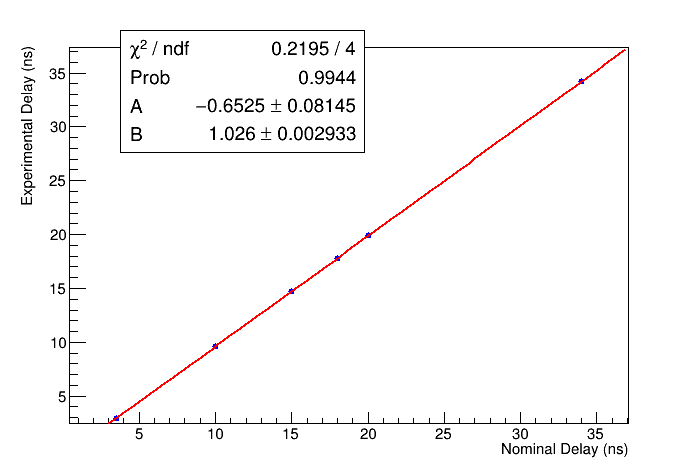
\includegraphics[width=.75\linewidth]{characterization/DelayLinearity}
	\caption{Relation between the nominal delay and experimental one. Error bars are calculated as the standard deviation of the $15$ measures (for each delay). Notwithstanding they are drawn, they are not visible due to their smallness.} \label{fig:delaylinearity}
\end{figure}
The accordance between data and the model \eqref{eq:linear} is excellent since
\begin{equation}
P_4\left(\chi^2\geq\chi_{obs}^2\right)=99.44\,\%
\end{equation}
but the fit results highlight a discrepancy with the ideal behavior $A_{id}=0$ and $B_{id}=1$ of order $8\sigma_A$ and $9\sigma_B$, respectively. Therefore, in the next analyses a correction to nominal delays due to a systematic error is mandatory:
\begin{equation} \label{correction}
\Delta t_{real} = A + B\cdot\Delta t_{nom}
\end{equation}
with
\begin{equation}
A=\left(-0.65\pm 0.08\right)\,\si{\nano\second}\qquad\quad B=\left(1.026\pm 0.003\right)
\end{equation}
The covariance matrix is
\begin{equation}
\textrm{C}_{AB}=\left(
\begin{array}{cc}
0.00663 & -0.00022\\\\
-0.00022 & 8.6\cdot 10^{-6}
\end{array}
\right).
\end{equation}

To conclude, from errors propagation formula, the uncertainty on $\Delta t_{real}$ will depend on the nominal delay in accordance with
\begin{equation} \label{err_correction}
\sigma_{\Delta t_{real}} = \sqrt{\sigma_A^2 + \left(\Delta t_{nom} \cdot \sigma_B\right)^2 + 2\Delta t_{nom}\cdot\sigma_{AB}  }.
\end{equation}

\subsection{Logic unit}
The programmable logic unit is a module used to make boolean operations between signals and it is employed in our experiment to perform coincidences between signals.
When configuring the electronics setup for the measurement of the muon lifetime, logic unit modules will be employed in order to perform start and stop topologies for the $\mu$ decay triggering. For this reason the characterization of the logic unit response is mandatory.

The logic unit is programmed in $\texttt{AND}$ mode in order to perform coincidences between signals. Therefore two NIM signals entering the 4-fold logic unit produce an output signal only if they are overlapped within a few ns.
Therefore, the aim of the logic unit characterization is to quantify the maximum time separation between two signals such that their overlapping is not enough to succeed in performing an $\texttt{AND}$ operation.\\

The characterization setup is shown in Figure \ref{logic_unit_1scinti}.
The pulse that is coming from the anode, if above the discriminator threshold, is divided along three different lines by means of a Fan-In/Fan-Out module.
One signal goes directly to a counter, which measures the total number of counts $N_{tot}$ for each measurement. 
The other two signals reach the logic unit along two different lines, i.e. passing through a delay unit or not. Finally the output signal of the logic unit is sent to a different channel of the counter, which counts the number of coincidences $N_{coinc}$ between the signals passing through the two lines, one delayed respect to the other.
In this configuration it is clear that, by means of the delay unit, one of the signal can be easily displaced in time. As a matter of fact, the measured value for $N_{coinc}$ depends on the delay which can be increased until the time separation among signals guarantees an overlapping sufficient to produce an output pulse. If the time shift becomes too large they are not recognized as overlapped anymore, consequently, since the two signals are not logically summed, the number of coincidences recorded at the counter changes abruptly.


\begin{figure}[!h]
	\centering
	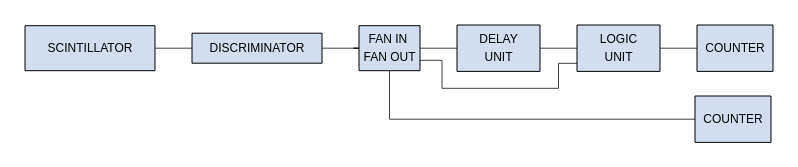
\includegraphics[width=\linewidth]{characterization/logic_unit_1scinti}
	\caption{Configuration employed during logic unit characterization with one scintillator.}
	\label{logic_unit_1scinti}
\end{figure}

The maximum time separation between coincident signals can be quantified comparing to what extent the counts measured in the two channels of the counter change when the delay is increased.
Therefore we can study the ratio between coincidences and total event counts as a function of the delay $\Delta t$ set on the delay unit, i.e.
\begin{equation} \label{eq:fermi_dirac}
f(\Delta t) = \frac{N_{coinc}(\Delta t)}{N_{tot}} .
\end{equation}

The sharp decreasing of the counts when the delay is increased can be parameterized by an empirical \emph{Fermi-Dirac}-like function which is used to perform the fit
\begin{equation} \label{eq:fermidirac}
f(\Delta t) = \frac{f_0}{1 + e^{k(\Delta t- t_0)}}
\end{equation}
where $f_0$ is the left-side asymptotic value of $f(\Delta t)$ for small $\Delta t$, $k$ is a constant and $t_0$ is the time at which $f(t_0) = 0.5 f_0$. As a matter of fact, the parameter $t_0$ corresponds to the discriminator output signal time-window (see Section \ref{discriminator}).\\

The width of the $f(t)$ distribution can be approximated from the tangent line to $f(t)$ evaluated at the point $t_0$
\begin{equation}
y(t) = - \frac{f_0}{4} k t + \frac{f_0}{2} \left(1 + \frac{k t_0}{2}\right)
\end{equation}
computing the distance between $t_0$ and the point $t^*$ at which the tangent line intersects the abscissa. $t^*$ is given by
\begin{equation}
t^* = \frac{2}{k} \left(1 + k \frac{t_0}{2}\right) .
\end{equation}
therefore the maximum time width $\delta_{T}$ of the logic unit within two signals are logically summed in $\texttt{AND}$ mode can be evaluated from the fit parameters as
\begin{equation}
\delta_{T} = 2 ( t^* - t_0 ) =  \frac{4}{k}.
\end{equation}

In order to reduce the systematic uncertainties, the real value of the delay with respect to the nominal one and its corresponding uncertainty have been computed by means of \eqref{correction} and \eqref{err_correction}, determined in the characterization of the delay unit.
Figure \ref{fig:fit_1scinti} shows the resulting fit of \eqref{eq:fermidirac} to the collected dataset. 
\begin{figure}[!htp]
	\centering
	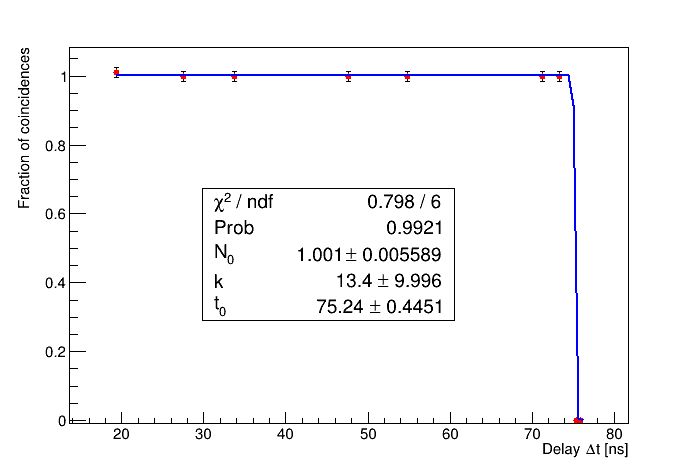
\includegraphics[width=.75\linewidth]{characterization/LogicUnit1}
	\caption{Logic unit characterization with a single split signal.} \label{fig:fit_1scinti}
\end{figure}
The estimated parameters are
\begin{equation}
\begin{array}{l}
f_0 = 1.001 \pm 0.006 \\
k = ( 13.397 \pm 9.996 ) \,  \si{ns^{-1}} \\
t_0 = ( 75.24 \pm 0.45 ) \,  \si{ns} .
\end{array}
\end{equation}
and the covariance matrix is
\begin{equation}
\textrm{C}=\left(
\begin{array}{ccc}
     3.12 \cdot 10^{-5}  &  5.19 \cdot 10^{-5}  &  2.38 \cdot 10^{-7} \\
    5.19 \cdot 10^{-5} &      99.93   &      4.27\\
    2.38 \cdot 10^{-7}  &       4.27   &    0.198
\end{array}
\right)
\end{equation}

The accordance between data and the model \eqref{eq:fermi_dirac} is excellent since
$P_6\left(\chi^2\geq\chi_{obs}^2\right)=99.21\,\%$.
It can be observed that the counts fall quite sharply around $\SI{75.2}{ns}$ and almost no counts are registered for delays greater than this.
The time width of the logic unit obtained is:
\begin{equation}
\delta_T = ( 0.299 \pm 0.223) \, \si{ns}
\end{equation}

The relative uncertainty obtained on $\delta_T$ is quite big $\left( \delta_{\delta_T} / \delta_T \sim 74.6 \%\right)$ since delay small enough to sample the step decreasing of the function were not experimentally found.\\

Almost the same strategy can be applied with two scintillators. 
The characterization setup is shown in Figure \ref{logic_unit_1scinti}:
\begin{figure}[!h]
	\centering
	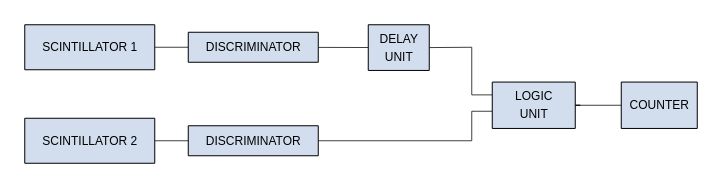
\includegraphics[width=\linewidth]{characterization/logic_unit_2scinti}
	\caption{Configuration employed during logic unit characterization with two scintillators.}
	\label{logic_unit_2scinti}
\end{figure}
in this configuration the signals come from two different scintillators and, before reaching the logic unit, one of them can be delayed with respect to the other by means of the delay module. Similarly, we can study the decreasing in the number of counts of coincident signals $N_{coinc}$ when the delay is increased.
The decreasing of the counts is parameterized by the empirical function
\begin{equation} \label{eq:fermi_dirac_1}
N_{coinc}(\Delta t) = \frac{N_0}{1 + e^{k(\Delta t- t_0)}}
\end{equation}
which is used to perform the fit.
Figure \ref{fig:fit_2scinti} shows the resulting fit of \eqref{eq:fermi_dirac_1} to the collected dataset. 
\begin{figure}[!htp]
	\centering
	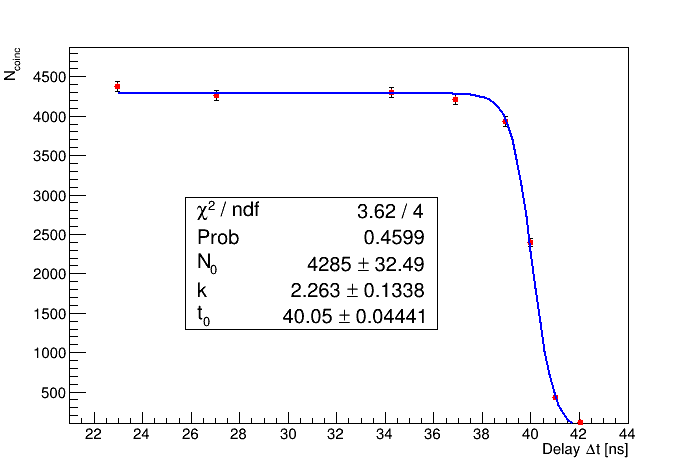
\includegraphics[width=.75\linewidth]{characterization/LogicUnit2}
	\caption{Logic unit characterization with signals from two scintillators.} \label{fig:fit_2scinti}
\end{figure}
The parameters estimated from the fit are
\begin{equation}
\begin{array}{l}
N_0 = ( 4.285 \pm 0.032 ) \cdot 10^3 \\
k = ( 2.26 \pm 0.13 ) \,  \si{ns^{-1}} \\
t_0 = ( 40.0514 \pm 0.044 ) \,  \si{ns}
\end{array}
\end{equation}

\noindent The covariance matrix is
\begin{equation}
\textrm{C}=\left(
\begin{array}{ccc}
1055.28  &     -1.22    &   -0.447 \\
-1.22   &     0.018   &    0.0017 \\
-0.447   &    0.0017  &     0.0019 \\
\end{array}
\right)
\end{equation}

The accordance between data and the model \eqref{eq:fermi_dirac_1} is satisfactory since
$P_4\left(\chi^2\geq\chi_{obs}^2\right)=45.98\,\%$.
The time width of the logic unit obtained is
\begin{equation}
\delta_T = ( 1.77 \pm 0.10 ) \, \si{ns}.
\end{equation}

The uncertainty on the measured value is quite small ($\delta_{\delta_T} / \delta_T \sim 6 \%$) since the fall in the number of counts is less abrupt and more data have been sampled in this region.
The different value for the estimated parameter $t_0$ in the two characterization schemes employed is simply due to a different choice of the discriminator channel, whose time-window are given in Table \ref{window}.
Moreover, when dealing with two scintillators, casual coincidences must be taken into account. The chance coincidence rate from uncorrelated input at rates $R_1$ and $R_2$ (i.e. event rates in the two scintillators)  is:
\begin{equation}
R_{chance} =  \tau R_1 R_2 \, \cite{Knoll}
\end{equation}
where $\tau$ is the time-window ($\tau = \SI{40}{ns}$). Here $R_1 = R_2 = \SI{40}{Hz}$ (see Section \ref{discriminator}), which gives $R_{chance} < 10^{-4}\si{Hz}$, which is negligible. 
Furthermore the decreasing of the number of counts is less abrupt since the signals come from two different scintillators, hence the effects of time jitter and amplitude walk become more important.

\subsection{Coincidence unit}
\documentclass[a4paper, 12pt]{report}
\usepackage{graphicx}

\begin{document}
	
\section{Electronics Modules Characterization}
\subsection{Coincidence Unit}
As the logic unit, the coincidence unit is a module used to make boolean operations between signals . The coincidence unit's imputs are logic pulses and the outputs are logic pulses if pulses appear at all imputs within a time interval (resolving time). In our experiment it is used(as the logic unit) to perform coincidences between signals.\\

The same approach used with the characterization of the logic unit can be applied to the coincidence unit.


The characterization setup is shown in Figure \ref{coinc_unit} and it is equivalent to the first set up for the logic unit . 

\begin{figure}[!h]
	\centering
	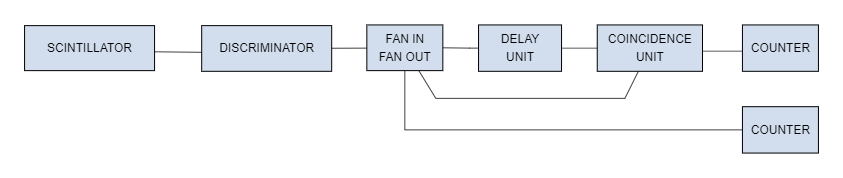
\includegraphics[width=\linewidth]{coinc_unit.png}
	\caption{Configuration employed during coincidence unit characterization}
	\label{coinc_unit}
\end{figure}


Also the fitting function(\eqref{eq:fermidirac}) and the way in which the errors are calculated are  always the same of the first characterization of the logic unit,thus the results can be shown directly. 


The estimated parameters are
\begin{eqnarray}
f_0 = 0.995 \pm 0.005\\
k = ( 20.936 \pm 9.790 ) \,  \si{ns^{-1}} \\
t_0 = ( 38.100 \pm 0.112 ) \,  \si{ns} .
\end{eqnarray}
and the covariance matrix is
\begin{equation}
\textrm{C}=\left(
\begin{array}{ccc}
     2.24 \cdot 10^{-5}  &  -1.39\cdot 10^{-2} &  -1.59 \cdot 10^{-4} \\
    -1.39 \cdot 10^{-2} &      95.84  &      0.98\\
    -1.59\cdot 10^{-4}  &       0.98   &    1.26\cdot 10^{-2} 
\end{array}
\right)
\end{equation}



The accordance between data and the model is excellent since $P_8\left(\chi^2\geq\chi_{obs}^2\right)=99.96\,\%$.
As in the  characterization of the logic unit it can be observed that  the counts fall quite sharply around a value of  delay and almost no counts are registered for delays greater than this.  
The value of this delay is almost \SI{38.1}{ns} and the time width of the coincidence unit obtained is: 

\begin{equation}
\delta_T = ( 0.191\pm 0.089 ) \, \si{ns}.
\end{equation}

The relative uncertainty obtained on $\delta_T$ is quite big $\left( \delta_{\delta_T} / \delta_T \sim 46.6 \%\right)$ since the decrease of the function is steep thus few data have been sampled in this region.   \\

\begin{figure}[!h]
	\centering
	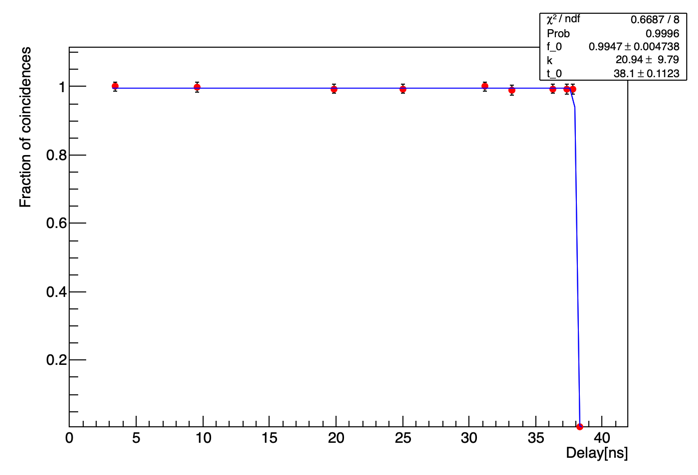
\includegraphics[width=\linewidth]{coinc_plot.png}
	\caption{Coincidence unit characterization}
	\label{coinc_plot}
\end{figure}



\end{document}

\subsection{Digitizer}
%\subsection{Digitizer} \label{sec:digitizer}

The last electronic device that has been characterized is the digitizer, which receives in input the signal from the electronic trigger chain and the signals from the scintillators. Indeed this instrument allows to convert the analog signal into a digital one and so it permits an offline analysis of the waveforms collected. Therefore using a function generator it has been possible to evaluate the linearity between the frequencies of the square signals given in input by the function generator and the frequencies obtained by the offline analysis of the data collected by the digitizer. As it can be seen in Figure \ref{fig:digitizer_linearity} the slope and the intercept of the fitting function are compatible with a linear trend as expected.
\begin{figure}[!htp]
	\centering
	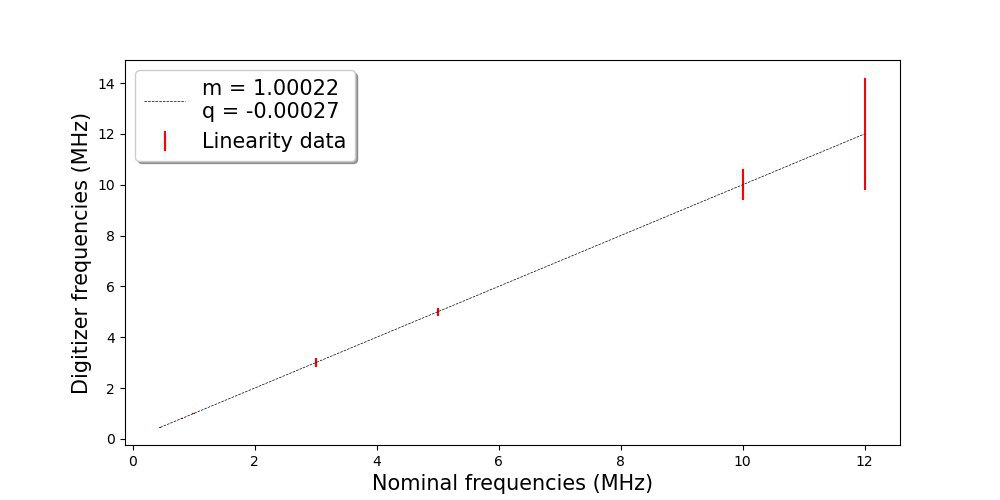
\includegraphics[width=.75\textwidth]{linearity_10}
	\caption{The data collected are reported in red and the fit function in a black dashed line. The errors are multiplied by a factor $10$ to highlight the small errors on the lower frequencies data.}
	\label{fig:digitizer_linearity}
\end{figure}
The data and the fit results are reported in Table \ref{tab:linearity_data} and first of all it is possible to see that the intercept of the fitting function is compatible with zero even if it is of no importance since exponential functions have been used the muon lifetime; in addition our data suggest a non-linearity smaller than $0.05\%$ and so it is possible to conclude that the non-linearity will be not taken into account in the later part of the experiment.
\begin{table}[!htp]
	\centering
	\begin{tabular}{rcc}
		\toprule
		\multicolumn{3}{c}{Fit results} \\
		\midrule
		Slope ($m$) &\multicolumn{2}{c}{$1.00022$} \\
		Intercept ($q$) &\multicolumn{2}{c}{$-0.00027$} \\
		Non-linearity ($\%$) &\multicolumn{2}{c}{$0.022$} \\
		\midrule
		\multicolumn{3}{c}{Data}\\
		\midrule
		Nominal Frequencies $\left[ \si{\mega\hertz}\right]$ & Measured Frequencies $\left[ \si{\mega\hertz}\right]$ & $\sigma \ \left[ \si{\mega\hertz}\right]$ \\
		\midrule
		$0.4500$ & $0.4500$ & $0.0004$ \\
		$0.5000$ & $0.5000$ & $0.0003$ \\
		$0.7000$ & $0.7000$ & $0.0008$ \\
		$0.8000$ & $0.8000$ & $0.0013$ \\
		$0.9900$ & $0.9901$ & $0.0020$ \\
		$1.0000$ & $1.0000$ & $0.0010$ \\
		$3.0000$ & $3.0001$ & $0.0169$ \\
		$5.0000$ & $5.0002$ & $0.0167$ \\
		$10.0000$ & $10.0004$ & $0.0607$ \\
		$12.0000$ & $12.0038$ & $0.2217$ \\
		\bottomrule
	\end{tabular}
	\caption{Fit results and recorded data.}
	\label{tab:linearity_data}
\end{table}

\section{Scintillators characterization}
The ideal detector should have various properties, in particular:
\begin{itemize}
	\item Perfect conversion of the kinetic energy of charged particles into light which must be detected with efficiency equal to $100\,\%$.
	\item Uniform light yield for each detector portion.
\end{itemize}
A further complication is given by the fact that the laboratory location is affected by a not-negligible natural background radiation which is mainly composed by photons.

As explained in Subsection~\ref{Mu-Sci}, plastic (organic) scintillators are preferred in timing measurements but, equally as any real detector, there are non-ideal behaviors that have to be recognized and taken into consideration before the subsequent muons lifetime measurements.

\subsection{Single-detector counting rates}
Background photons usually belong to energy ranges lower than the mean $\mu$-energy (at the ground) of about $\SI{4}{\giga\electronvolt}$, thus the employment of a discriminator module is a reasonable way to suppress them (the instruments configuration is shown in Figure \ref{fig:single-rate}).
\begin{figure}[!h]
	\centering
	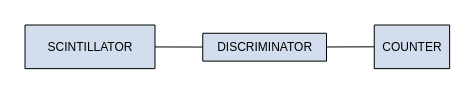
\includegraphics[width=.8\linewidth]{characterization/rate}
	\caption{Single-detector counting rates configuration.}
	\label{fig:single-rate}
\end{figure}

As a first step towards excluding $\gamma$-background, a study of both discriminator threshold and photo-multiplier bias voltages is carried out by taking into account one single detector at a time.\\

At fixed bias voltage, the expected behavior is the following: the higher threshold tension is, the lower counting rate is, until a \emph{plateau} is reached, when (ideally) all signals generated by background photons have been rejected and only muons are detected.\\
\begin{figure}[!htp]
	\centering
	\begin{subfigure}{.5\linewidth}
		\centering
		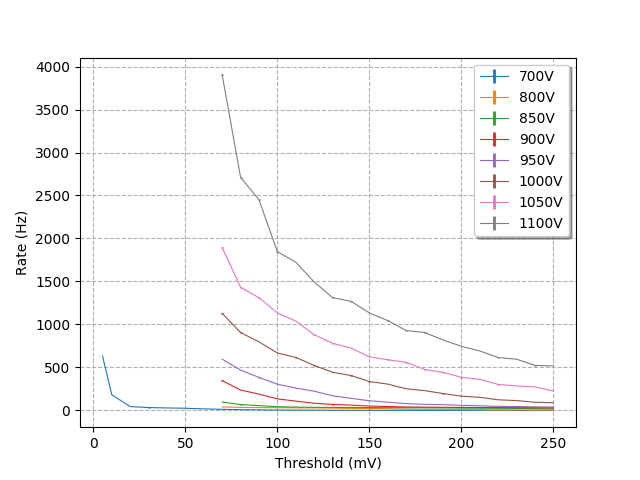
\includegraphics[width=\linewidth]{characterization/rate_threshold_caronte}
		\caption{\emph{Caronte}.} 
		\label{subfig:rt_caronte}
	\end{subfigure}\hfill
	\begin{subfigure}{.5\linewidth}
		\centering
		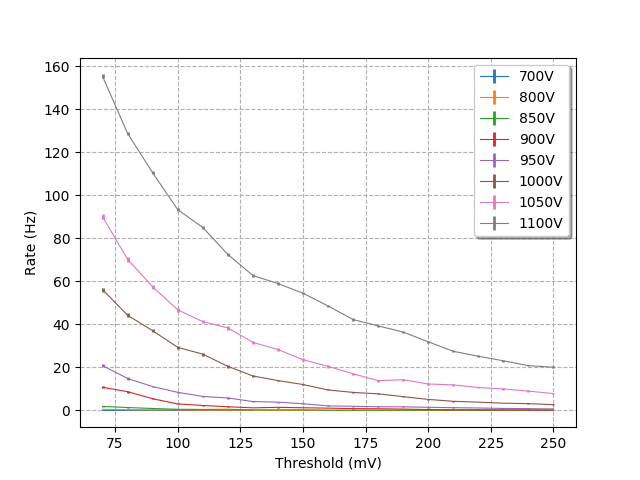
\includegraphics[width=\linewidth]{characterization/rate_threshold_cerbero}
		\caption{\emph{Cerbero}.} 
		\label{subfig:rt_cerbero}
	\end{subfigure}\hfill
	\begin{subfigure}{\linewidth}
		\centering
		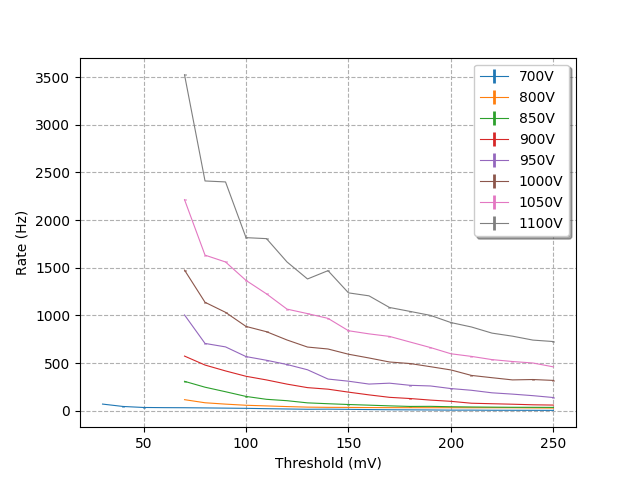
\includegraphics[width=.5\linewidth]{characterization/rate_threshold_minosse}
		\caption{\emph{Minosse}.} 
		\label{subfig:rt_minosse}
	\end{subfigure}
	\caption{Rate as a function of discriminator threshold tension, at fixed bias voltages. Errors on rates are calculated as $\sqrt{N}/t$, according to \emph{Poisson} probability distribution.} 
	\label{fig:rt}
\end{figure}

Figure \ref{fig:rt} highlights a more complicated trend, which is far from clarifying a suitable combination of threshold and bias voltages. Of course the most significant analysis will be performed concerning the detection efficiency (see Subsection \ref{sub:detection_eff}), but some aspects are worth considering, in fact it is important to note that the threshold can not be increased as desired since, after a certain value, in addition to photons, muons are rejected too. This behavior is clear if taking into consideration the obtained counting rates lower than the $\approx\SI{40}{\hertz}$ expected muons one.

By comparing \emph{Caronte} (Figure \ref{subfig:rt_caronte}) and \emph{Minosse} (Figure \ref{subfig:rt_minosse}) with \emph{Cerbero} (Figure \ref{subfig:rt_cerbero}), we can predict that the latter is definitely less efficient than the former detectors. Moreover, when working at low bias voltages (e.g. $\SI{700}{\volt}$), even the lowest considered thresholds are sufficient to cut most of the signal and we are legitimated to suspect that higher bias tensions should be preferred.\\
\begin{figure}[!htp]
	\centering
	\begin{subfigure}{.5\linewidth}
		\centering
		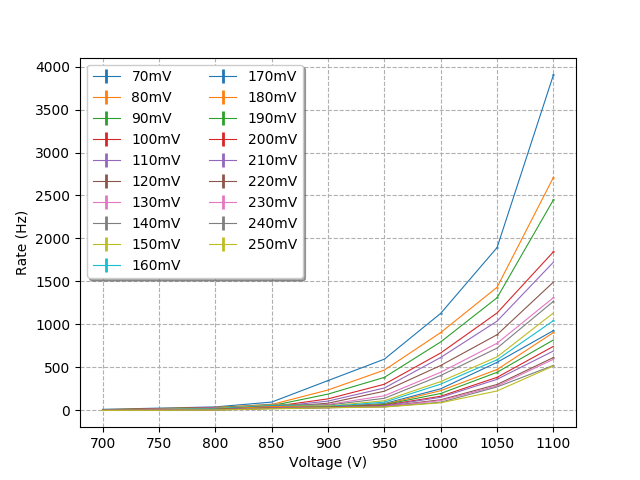
\includegraphics[width=\linewidth]{characterization/rate_bias_caronte}
		\caption{\emph{Caronte}.} 
		\label{subfig:rb_caronte}
	\end{subfigure}\hfill
	\begin{subfigure}{.5\linewidth}
		\centering
		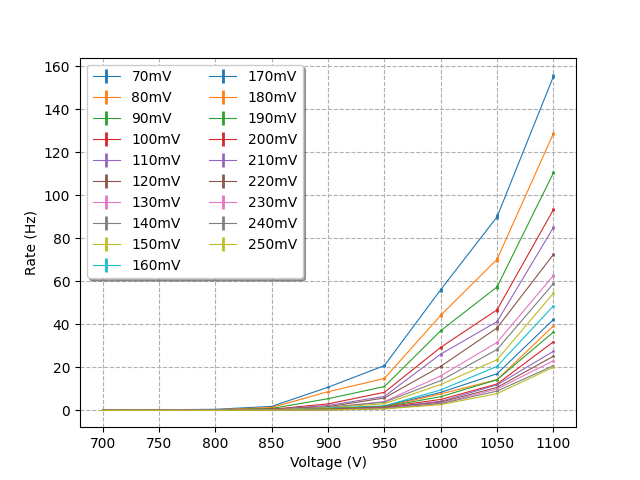
\includegraphics[width=\linewidth]{characterization/rate_bias_cerbero}
		\caption{\emph{Cerbero}.} 
		\label{subfig:rb_cerbero}
	\end{subfigure}\hfill
	\begin{subfigure}{.5\linewidth}
		\centering
		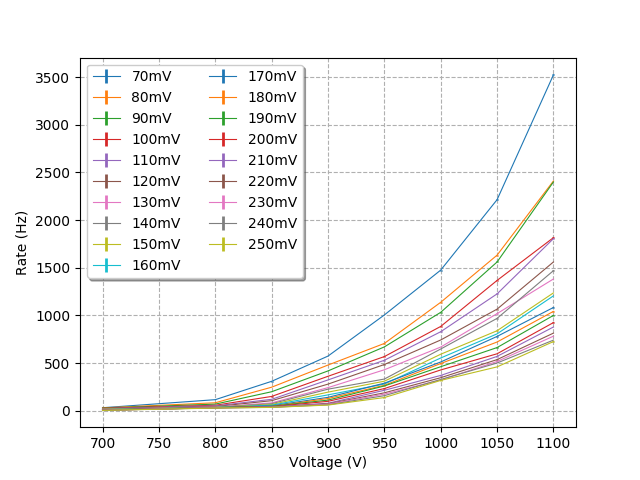
\includegraphics[width=\linewidth]{characterization/rate_bias_minosse}
		\caption{\emph{Minosse}.} 
		\label{subfig:rb_minosse}
	\end{subfigure}
	\caption{Rate as a function of bias voltage, at fixed discriminator thresholds. Errors on rates are calculated as $\sqrt{N}/t$, according to \emph{Poisson} probability distribution.} 
	\label{fig:rb}
\end{figure}

\begin{figure}[!htp]
	\centering
	\begin{subfigure}{\linewidth}
		\centering
		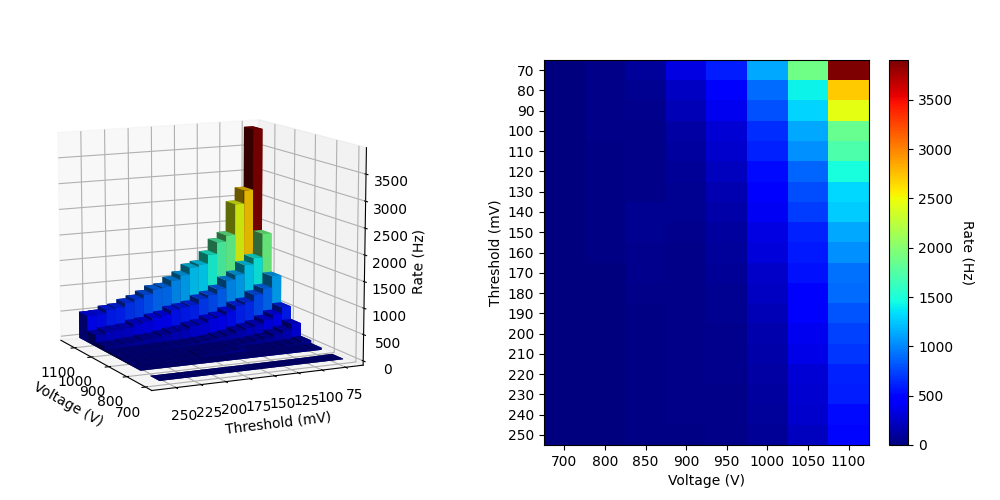
\includegraphics[width=.9\linewidth]{characterization/3d_caronte}
		\caption{\emph{Caronte}.} 
		\label{subfig:3d_caronte}
	\end{subfigure}\hfill
	\begin{subfigure}{\linewidth}
		\centering
		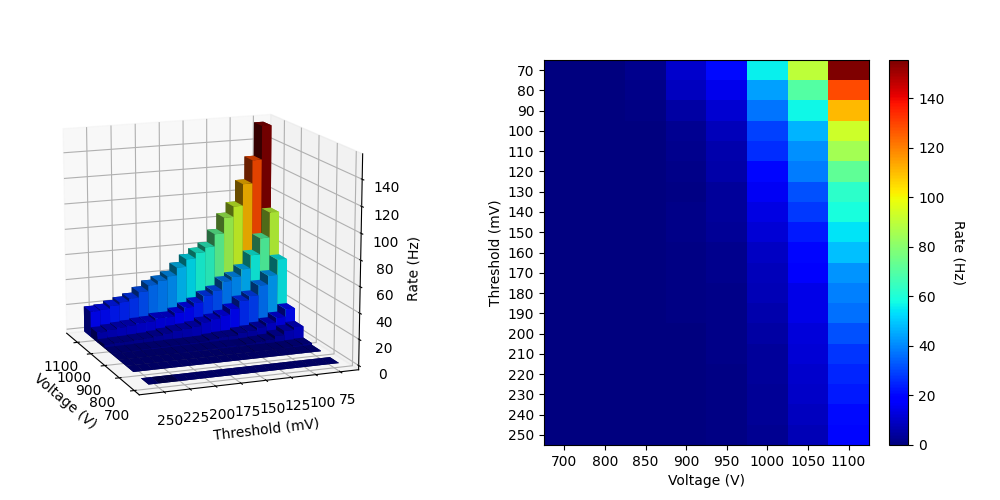
\includegraphics[width=.9\linewidth]{characterization/3d_cerbero}
		\caption{\emph{Cerbero}.} 
		\label{subfig:3d_cerbero}
	\end{subfigure}\hfill
	\begin{subfigure}{\linewidth}
		\centering
		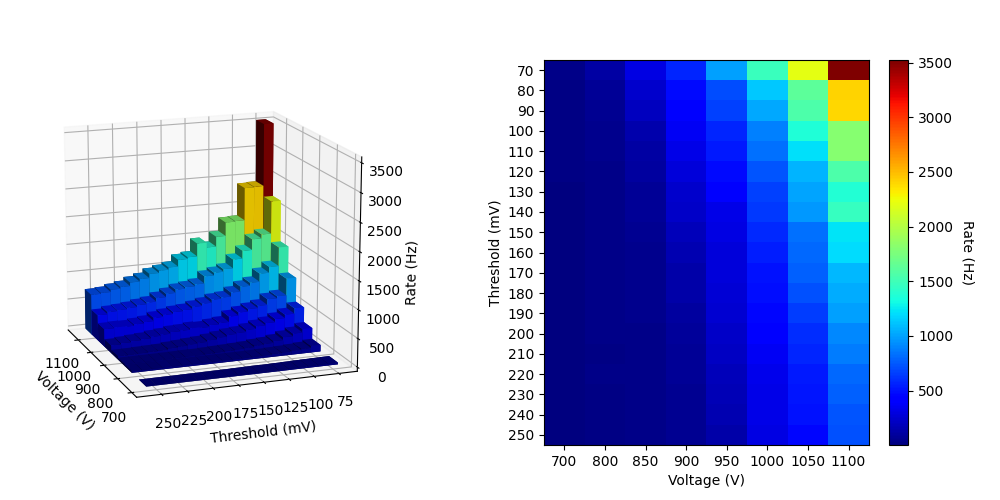
\includegraphics[width=.9\linewidth]{characterization/3d_minosse}
		\caption{\emph{Minosse}.} 
		\label{subfig:3d_minosse}
	\end{subfigure}
	\caption{Rate as a function of threshold and bias voltages. 3D plot (on the left) and heat-map (on the right).} 
	\label{fig:3d}
\end{figure}
%\begin{figure}
%	\ContinuedFloat
%	\begin{subfigure}{\linewidth}
%		\centering
%		\includegraphics[width=.7\linewidth]{characterization/3d_mino
%		e}
%		\caption{\emph{Minosse}.} 
%		\label{subfig:3d_minossex}
%	\end{subfigure}
%\end{figure}

Instead, a study of single-detector counting rates at fixed discriminator threshold is represented in Figure \ref{fig:rb}. Data shown in Figure \ref{fig:rt} and \ref{fig:rb} are then combined in Figure \ref{fig:3d}, allowing an overall sight.\\

As above-mentioned, the interesting feature that has to be studied is the efficiency, however the single-detector counting rates are useful, meaning that they can give a first rough idea of what is the region of voltages from which is worth beginning the efficiencies analysis. In fact, by observing the zoomed-in Figure \ref{fig:zoomed} plots, we can identify a flattening behavior in the neighborhood of $\sim \SI{40}{\hertz}$ for \emph{Caronte} and  \emph{Minosse}, whilst  \emph{Cerbero} does not exhibit a similar trend, justifying the suspected low detection efficiency.

\begin{figure}[!htp]
	\centering
	\begin{subfigure}{.5\linewidth}
		\centering
		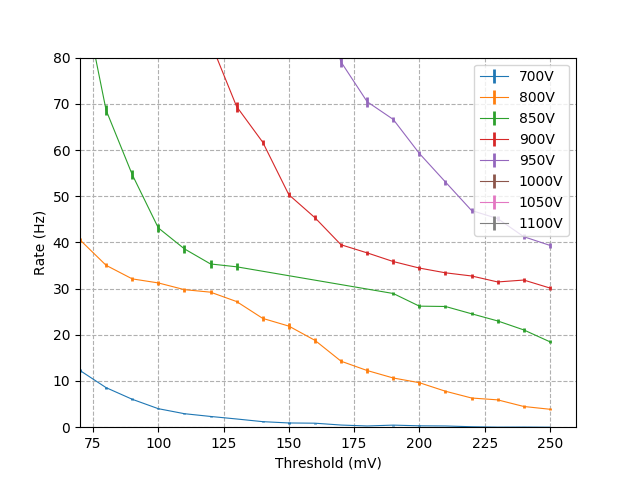
\includegraphics[width=\linewidth]{characterization/rate_threshold_caronte_zoomed}
		\caption{\emph{Caronte}.} 
		\label{subfig:zoomed_caronte}
	\end{subfigure}\hfill
	\begin{subfigure}{.5\linewidth}
		\centering
		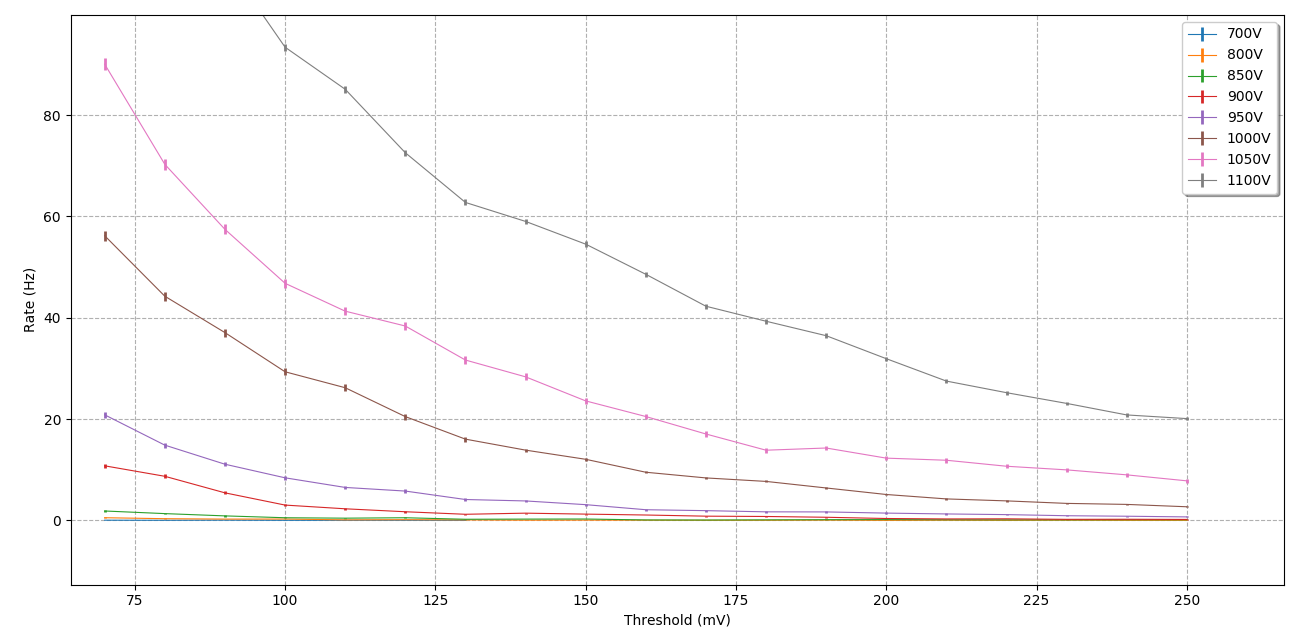
\includegraphics[width=\linewidth]{characterization/rate_threshold_cerbero_zoomed}
		\caption{\emph{Cerbero}.} 
		\label{subfig:zoomed_cerbero}
	\end{subfigure}\hfill
	\begin{subfigure}{\linewidth}
		\centering
		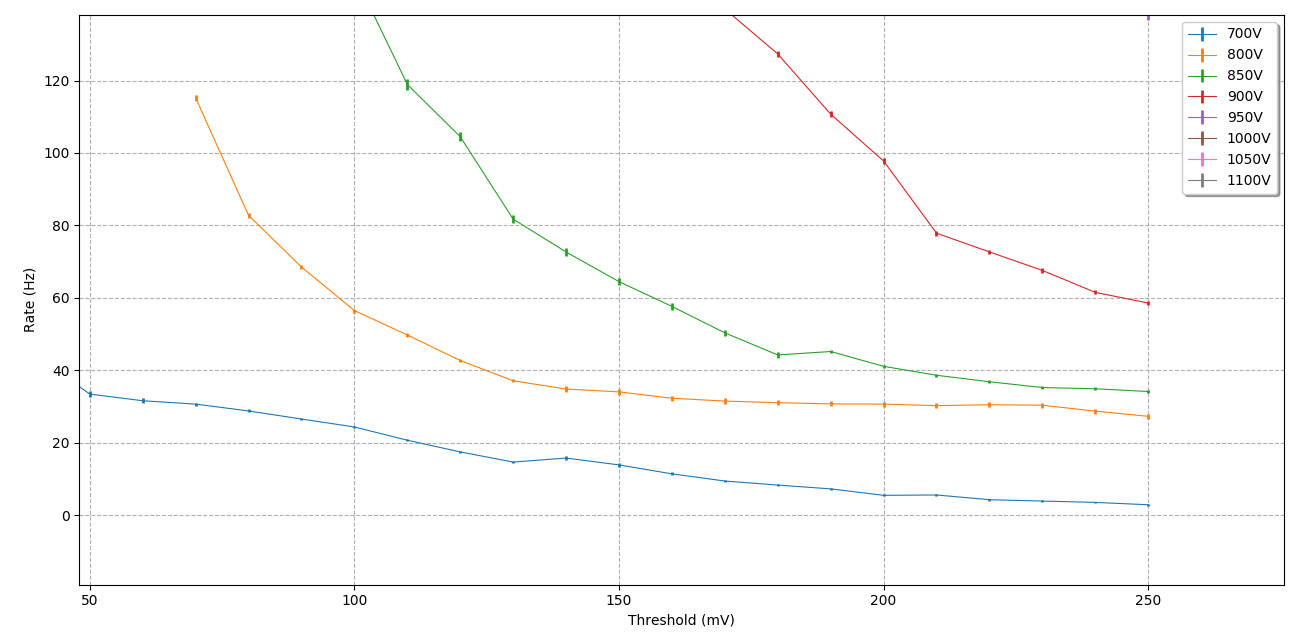
\includegraphics[width=.5\linewidth]{characterization/rate_threshold_minosse_zoomed}
		\caption{\emph{Minosse}.} 
		\label{subfig:zoomed_minosse}
	\end{subfigure}
	\caption{Rate as a function of discriminator threshold tension, at fixed bias voltages. Magnification on plateau areas of Figure \ref{fig:rb}.} 
	\label{fig:zoomed}
\end{figure}



\subsection{Detection efficiency} \label{sub:detection_eff}

Of course, a condition where detectors work with the highest efficiencies is fundamental and thus a setup that is suitable for efficiency estimation has to be prepared.
\begin{figure}[!h]
	\centering
	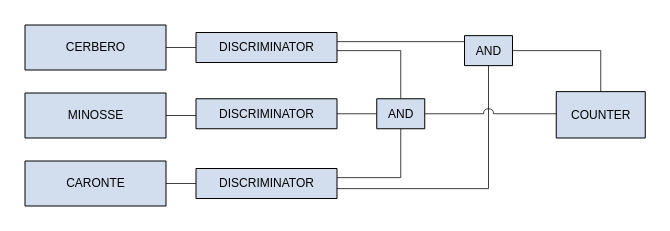
\includegraphics[width=.8\linewidth]{characterization/efficiency}
	\caption{Efficiency studies setup.}
	\label{fig:eff-setup}
\end{figure}
With an aligned geometry (where the three $80\times 30$ cm scintillators are one above the other) the detection efficiency of the middle detector can be easily calculated as
\begin{equation}
\varepsilon = \frac{N_{triple}}{N_{double}}
\end{equation}
where $N_{double}$ is the number of coincidences between the upper scintillator and the lower one, instead $N_{triple}$ is given by the coincidence of all detector signals. Figure \ref{fig:eff-setup} is a pictorial diagram of the instrumentation setup. The \texttt{AND} ports are realized by means of a programmable logic unit.\\
\begin{figure}[!bp]
	\centering
	\begin{subfigure}{.5\linewidth}
		\centering
		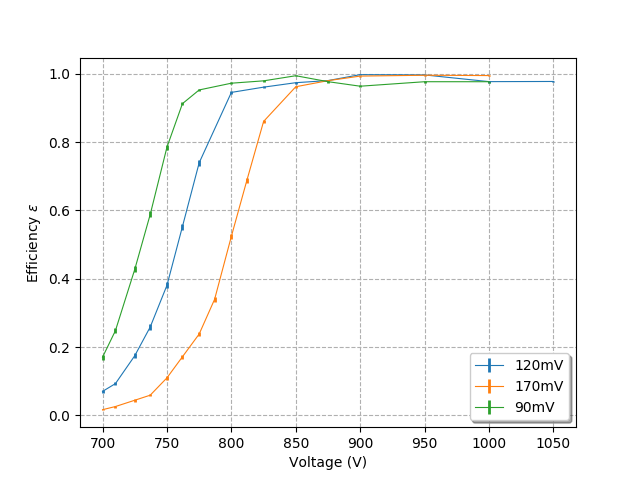
\includegraphics[width=\linewidth]{characterization/eff_caronte}
		\caption{\emph{Caronte}.} 
		\label{subfig:eff_caronte}
	\end{subfigure}\hfill
	\begin{subfigure}{.5\linewidth}
		\centering
		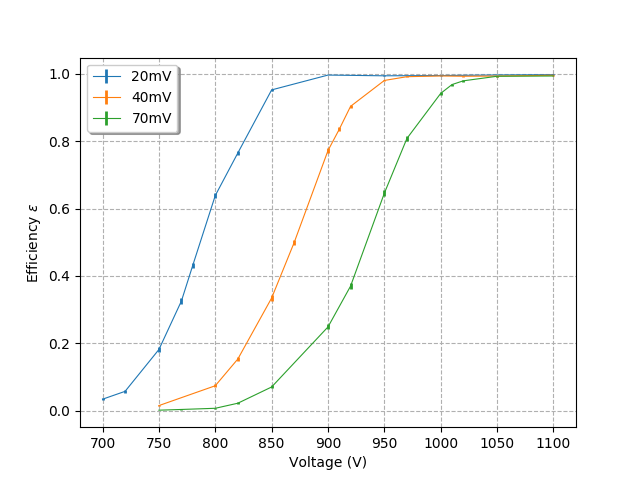
\includegraphics[width=\linewidth]{characterization/eff_cerbero}
		\caption{\emph{Cerbero}.} 
		\label{subfig:eff_cerbero}
	\end{subfigure}\hfill
\end{figure}
\begin{figure}[!ht]
	\centering
	\ContinuedFloat
	\begin{subfigure}{.5\linewidth}
	\centering
	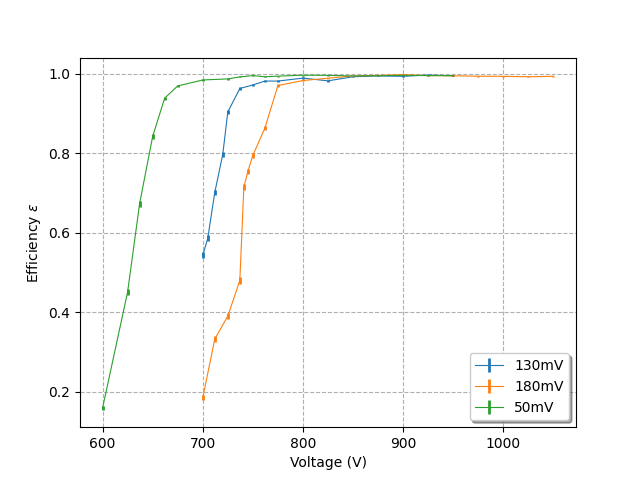
\includegraphics[width=\linewidth]{characterization/eff_minosse}
	\caption{\emph{Minosse}.} 
	\label{subfig:eff_minosse}
	\end{subfigure}
	\caption{Detection efficiencies.} 
	\label{fig:eff}
\end{figure}

Figure \ref{fig:zoomed} highlights which configurations of bias and threshold voltages are advisable in order to work mainly with muons and be left with a little-to-no $\gamma$-background, therefore the scintillators efficiencies represented in Figure \ref{fig:eff}  (data are contained in Appendix \ref{app:eff}) give a clear information of the bias-threshold setup that has to be avoided so as to guarantee the largest light yield.\\

Concerning the efficiency estimation from a statistical perspective, and considering that
\begin{equation}\label{eq:binomial}
N_{triple}=N_{double}\cdot\varepsilon
\end{equation}
the number of triple counts is nothing but the result of \emph{Bernoulli} trial where $N_{double}$ is the total number of trials and $\varepsilon$ is the probability of success, i.e. the particle is effectively detected by the middle detector. Therefore, the uncertainty on $N_{triple}$ is due to the binomial probability distribution:
\begin{equation}
\sigma_{triple}=\sqrt{N_{double}\cdot\varepsilon\left(1-\varepsilon\right)}
\end{equation}
and, according to propagation of errors formula, we end up with
\begin{equation}\label{eq:eff_err}
\sigma_{\varepsilon}=\sqrt{\frac{\varepsilon\left(1-\varepsilon\right)}{N_{double}}}=\displaystyle\frac{1}{N_{double}}\sqrt{N_{triple}\left(1-\frac{N_{triple}}{N_{double}}\right)}
\end{equation}
\eqref{eq:eff_err} is the expression which error bars on efficiency have been conveniently calculated with.\\

Finally, the chosen configuration is summed up in Table \ref{tab:bt-setup}.
\begin{table}[!hb]
	\centering
	\begin{tabular}{r|ccc}
		\toprule
		Detector&Bias Voltage (V)&Threshold tension (mV)&Efficiency $\varepsilon$\\
		\midrule
		\emph{Caronte} & $900$ & $170$ & $0.9937\pm 0.0013$\\
		\emph{Cerbero} & $1000$ & $40$ & $0.9938\pm 0.0013$\\
		\emph{Minosse} & $850$ & $180$ & $0.9948\pm 0.0011$\\
		\bottomrule
	\end{tabular}
	\caption{Bias-threshold setups that have been chosen for physics measurements.}
	\label{tab:bt-setup}
\end{table}


\subsection{Uniformity of light yield}

\label{sec:uniformity}

In the previous section an overall efficiency has been calculated for each scintillator, but we are interested in understanding if the detector light yield keeps itself unvaried through different portions, thus the conclusive analyses in terms of the detectors characterization are the uniformity studies.\\

\begin{figure}[!hbtp]
	\centering
	\begin{subfigure}{.3\linewidth}
		\centering
		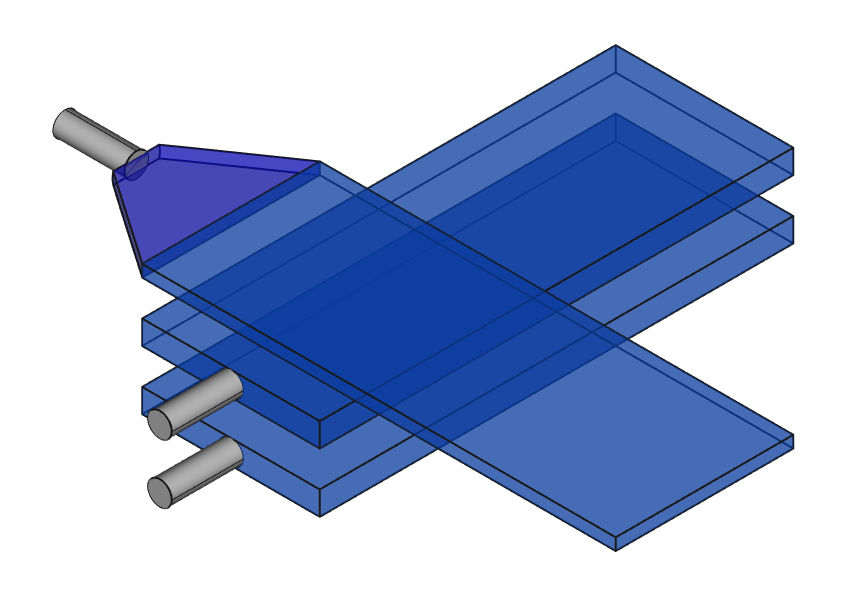
\includegraphics[width=\linewidth]{characterization/uniformity1}
		\caption{First layout.} 
		\label{subfig:uniformity1}
	\end{subfigure}\hfill
	\begin{subfigure}{.3\linewidth}
		\centering
		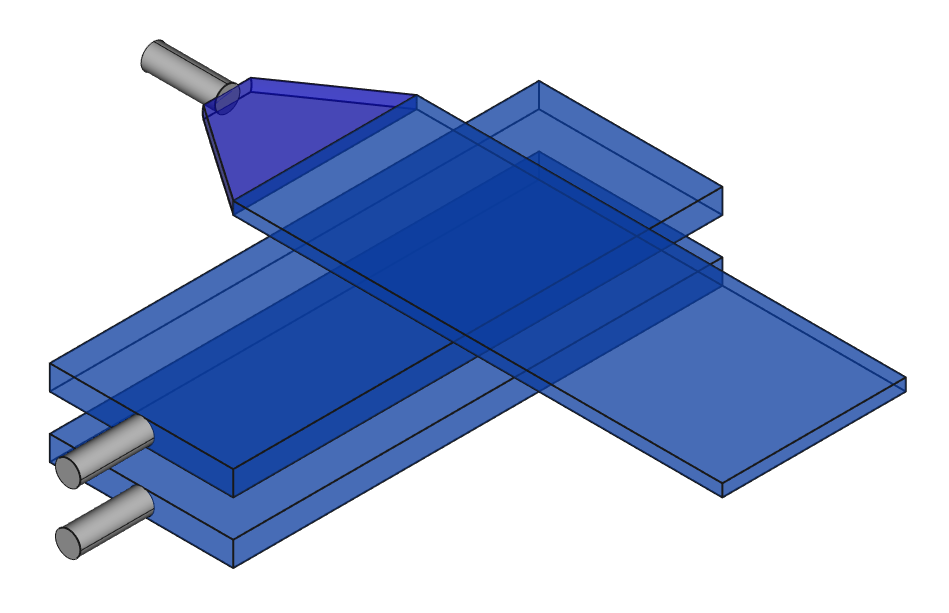
\includegraphics[width=\linewidth]{characterization/uniformity2}
		\caption{Second layout.} 
		\label{subfig:uniformity2}
	\end{subfigure}\hfill
	\begin{subfigure}{.3\linewidth}
		\centering
		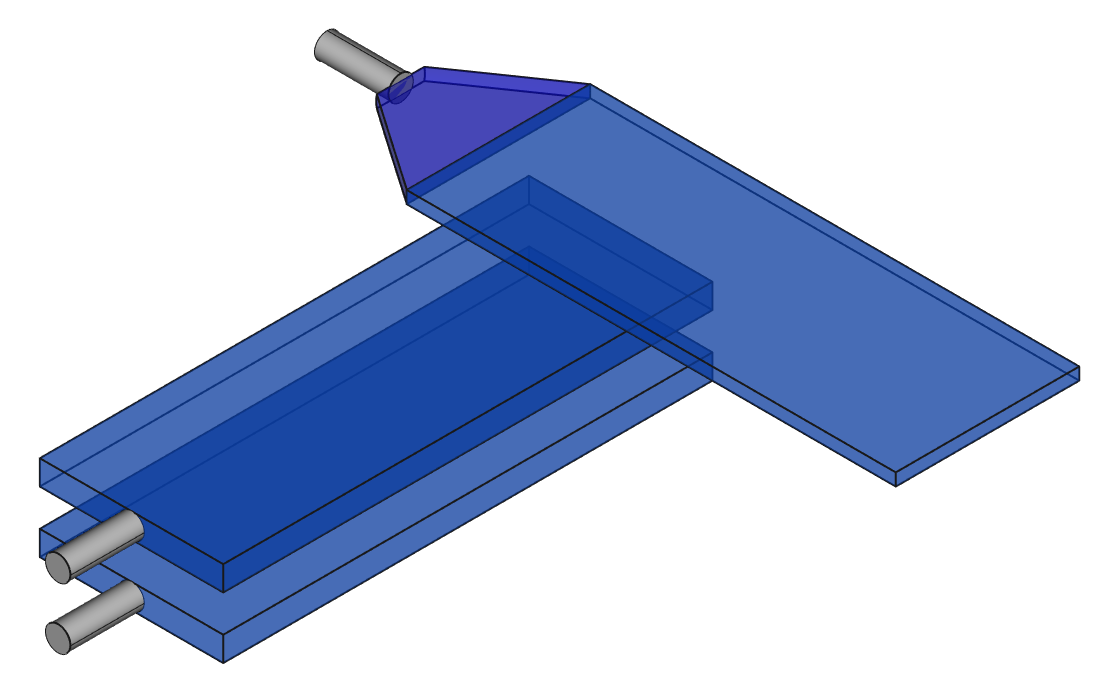
\includegraphics[width=\linewidth]{characterization/uniformity3}
		\caption{Third layout.} 
		\label{subfig:uniformity3}
	\end{subfigure}
	\caption{Detectors setup during uniformity studies. From below: \emph{Caronte}, \emph{Minosse}, \emph{Cerbero}.}
	\label{fig:uniformity}
\end{figure}

The instrumentation setup is unchanged with respect to Figure \ref{fig:eff-setup}, however the geometrical layout is no longer aligned, but organized for a specific area study, as Figure \ref{fig:uniformity} illustrates.\\

Before presenting the results of the analyses we call attention to the fact that efficiency can not be calculated as the ratio of $N_{triple}$ to  $N_{double}$ anymore, as a consequence of a geometrical effect previously explained in Section \ref{sec:uniformity_studies}. Therefore, the correct formula is \eqref{eq:eff_correct} where $\varepsilon_{g}$ comes from the Monte Carlo simulations, whose results are collected in Table \ref{tab:err-effg}.\\

The errors take into account both the statistical nature due to the binomial probability distribution of $N_{triple}$ and the systematical uncertainty estimated on $\varepsilon_{g}$ (see Table \ref{tab:err-effg}), hence we have $\varepsilon\pm \sigma_{\varepsilon}^{stat} \pm \sigma_{\varepsilon}^{sys}$ where
\begin{equation}
\sigma_{\varepsilon}^{stat}=\displaystyle\frac{1}{\varepsilon_{g}\cdot N_{double}}\sqrt{N_{triple}\left(1-\frac{N_{triple}}{\varepsilon_{g}\cdot N_{double}}\right)}
\end{equation}
and
\begin{equation}
\sigma_{\varepsilon}^{sys}=\frac{N_{triple}\cdot\sigma_{\varepsilon_{g}}}{\varepsilon_{g}^2\cdot N_{double}}
\end{equation}

\begin{table}[!bht]
	\centering
	\begin{tabular}{r|ccc}
		\toprule
		&$N_{triple}$&$N_{double}$&$\varepsilon\pm\sigma_{\varepsilon}^{stat}\pm\sigma_{\varepsilon}^{sys}$\\
		\midrule
		Layout 1 &$4975$ & $5406$ & $0.979\pm 0.002 \pm 0.005$\\
		Layout 2 &$5332$ & $5746$	& $0.9893\pm 0.0014 \pm 0.005$\\
		Layout 3 &$3473$ & $3947$ & $0.987\pm 0.002 \pm 0.010$\\
		\bottomrule	
	\end{tabular}
	\caption{Layouts efficiencies, \emph{Caronte}.}\label{tab:unif_caronte}
\end{table}
\begin{table}[!hbt]
	\centering
	\begin{tabular}{r|ccc}
		\toprule
		&$N_{triple}$&$N_{double}$&$\varepsilon\pm\sigma_{\varepsilon}^{stat}\pm\sigma_{\varepsilon}^{sys}$\\
		\midrule
		Layout 1 &$4320$ & $4803$ & $0.9928\pm 0.0013\pm 0.006$\\
		Layout 2 &$4991$ & $5606$	& $0.9848\pm 0.0017\pm 0.006$\\
		Layout 3 &$3455$ & $4081$ & $0.9960\pm 0.0011\pm 0.009$\\
		\bottomrule	
	\end{tabular}
	\caption{Layouts efficiencies, \emph{Cerbero}.}\label{tab:unif_cerbero}
\end{table}
\begin{table}[!tb]
	\centering
	\begin{tabular}{r|ccc}
		\toprule
		&$N_{triple}$&$N_{double}$&$\varepsilon\pm\sigma_{\varepsilon}^{stat}\pm\sigma_{\varepsilon}^{sys}$\\
		\midrule
		Layout 1 &$4916$ & $5279$ & $0.9907\pm 0.0014\pm 0.005$\\
		Layout 2 &$5428$ & $5837$	& $0.9914\pm 0.0013\pm0.005$\\
		Layout 3 &$3768$ & $4356$ & $0.970\pm 0.003\pm 0.010$\\
		\bottomrule	
	\end{tabular}
	\caption{Layouts efficiencies, \emph{Minosse}.}\label{tab:unif_minosse}
\end{table}


For each scintillator, the resulting efficiencies (Table \ref{tab:unif_caronte}, \ref{tab:unif_cerbero} and \ref{tab:unif_minosse}) reveal normalized deviations that span in the range $0.1$-$1.8$ (see Table \ref{tab:norm_dev}). \emph{Cerbero} results are compatible with the hypothesis of a uniform detector and are in agreement with the efficiency estimated in the aligned setup.  
Notwithstanding the \emph{Caronte} and \emph{Minosse} results could suggest the evidence of some non-uniformity, we can see that efficiencies are systematically underestimated with respect to the overall ones showed in Table \ref{tab:bt-setup}, therefore it is clear that the geometrical weight estimated by means of the Monte Carlo procedure is not enough to cure the inconsistencies due to systematic errors encountered with these detectors.

\begin{table}[!hbt]
	\centering
	\begin{tabular}{r|ccc}
		\toprule
		Detector&$t_{12}$&$t_{13}$&$t_{23}$\\
		\midrule
		Caronte &$1.4$ & $1.4$ & $0.2$\\
		Cerbero &$0.9$ & $0.3$ & $1.0$\\
		Minosse &$0.1$ & $1.8$ & $1.8$\\
		\bottomrule	
	\end{tabular}
	\caption{Normalized deviations calculated as $t_{ij}=\left|\varepsilon_{i}-\varepsilon_{j}\right|/\sqrt{\sigma_{\varepsilon_{i}}^2+\sigma_{\varepsilon_{j}}^2}$ where $i,j$ are referred to layouts.}\label{tab:norm_dev}
\end{table}

The evidence of an additional systematic error\footnote{Since the distance between scintillators with \emph{Caronte} in the middle position is the same of \emph{Minosse} as middle detector, we could suspect that a mistake has been made while measuring the distances.} we have not identified led us to make one extra uniformity measurements session, by means of a new littler $27.5\times \SI{8.3}{cm}$ plastic scintillator, whose bias voltage and discrimination threshold tension have been set to $\SI{1550}{V}$ (according to the manufacturer recommendations) and $\SI{40}{mV}$, respectively. The acquisition time is $20$ minutes, in order to collect sufficient counts and reduce the statistical uncertainty.
\begin{figure}[!htb]
	\centering
	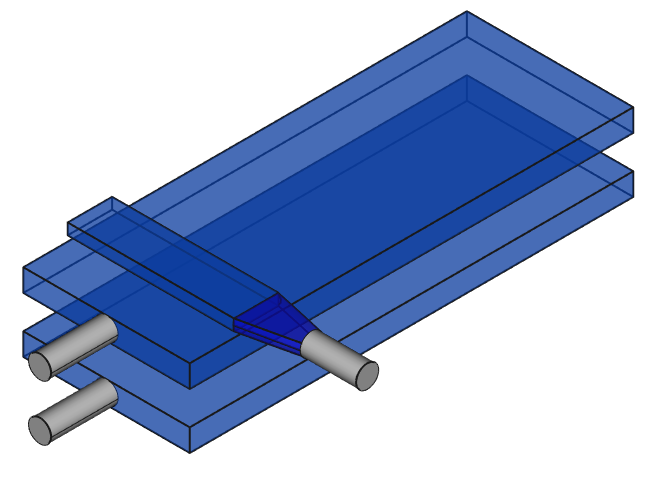
\includegraphics[width=.29\linewidth]{characterization/Paletta}
	\caption{Detectors setup during fine uniformity studies. From below: \emph{Caronte}, \emph{Minosse}, ``new'' scintillator.} \label{fig:fine_unif}
\end{figure}

This part of the analysis has been carried out only referring to \emph{Minosse} (the geometrical setup is shown in Figure \ref{fig:fine_unif}). Table \ref{tab:fine_eff} shows the results of the study, whose graphical representation is given in Figure \ref{fig:fine_eff}.\\

\begin{table}
	\centering
	\begin{tabular}{r|ccc}
		\toprule
		&$N_{triple}$&$N_{double}$&Efficiency $\varepsilon$\\
		\midrule
		Area 1 & $1312$	& $1314$ &	$0.9985\pm	0.0011$\\
		Area 2 & $1379$	& $1382$ &	$0.9978\pm	0.0013$\\
		Area 3 & $1184$	& $1188$ &	$0.9966\pm	0.0017$\\
		Area 4 & $1519$	& $1521$ &	$0.9987\pm	0.0009$\\
		Area 5 & $1584$	& $1589$ &	$0.9969\pm	0.0014$\\
		Area 6 & $2352$	& $2352$ &	$1.0000\pm	0.0000$\\
		Area 7 & $2334$	& $2336$ &	$0.9991\pm	0.0006$\\
		Area 8 & $1917$	& $1920$ &	$0.9984\pm	0.0009$\\
		Area 9 & $1655$	& $1660$ &	$0.9970\pm	0.0014$\\
		\bottomrule
	\end{tabular}
    \caption{\emph{Minosse} efficiencies during fine uniformity studies. The uncertainty on $\varepsilon$ has been computed according to \eqref{eq:eff_err}.} \label{tab:fine_eff}
\end{table}

Except for too small errors on the efficiencies which may cause possible discrepancies, we do not observe problematic behaviors in any portion of the detector.

\begin{figure}[!bht]
	\centering
	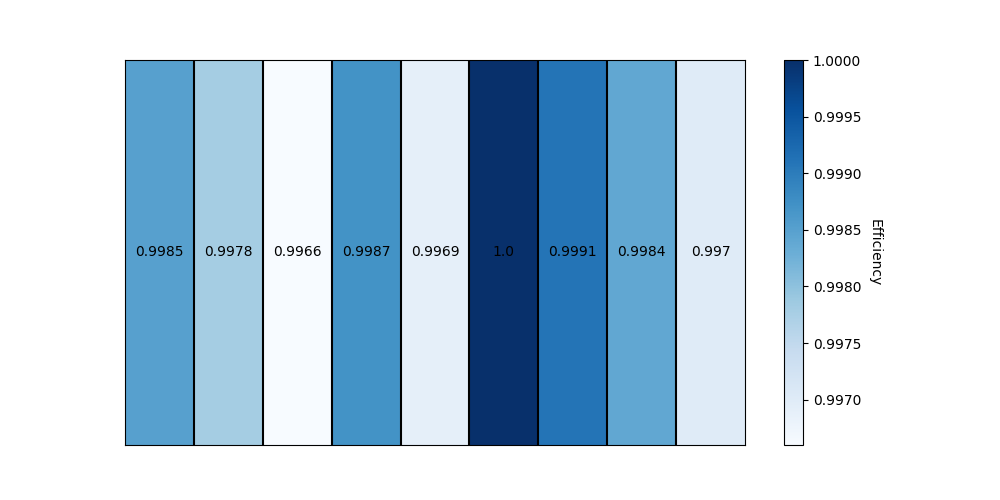
\includegraphics[width=.8\linewidth]{characterization/fine_uniformity_minosse}
	\caption{\emph{Minosse} efficiencies during fine uniformity studies.} \label{fig:fine_eff}
\end{figure}
